\documentclass[margin=2pt]{standalone}
\usepackage[table]{xcolor}
\usepackage[utf8]{inputenc}
\usepackage[T1]{fontenc}

\usepackage{tikz}
\usepackage{helvet}
\usepackage{amsmath}

\renewcommand\familydefault\sfdefault

% Use \phantom to hide text for exams
\renewcommand{\phantom}{}

\newcommand{\lCPU}{CPU}
\newcommand{\lPageTable}{Tabulka \phantom{stránek}}
\newcommand{\lLimit}{LA > Limit?}
\newcommand{\lLimitError}{Chyba narušení\\ochrany}
\newcommand{\lMemory}{Paměť} % \phantom{}
\newcommand{\lFAP}{FAP}
\newcommand{\lAddressLogical}{\phantom{Logická}\\{adresa}}
\newcommand{\lAddressPhysical}{\phantom{Fyzická}\\{adresa}}
\newcommand{\lRegLimit}{\phantom{Limitní}\\(mezní)\\registr}
\newcommand{\lRegBase}{Realokační\\(\phantom{bázový})\\registr}
\newcommand{\PhysicalMemory}{Fyzická paměť}

\usetikzlibrary{intersections, shapes.arrows, spath3, shapes.geometric, fit, backgrounds, calc, tikzmark, decorations.pathreplacing, angles, quotes}

\definecolor{themeBlue}{RGB}{1, 103, 143}
\definecolor{themeOrange}{RGB}{221, 109, 16}
\definecolor{themeTeal}{RGB}{18, 54, 69}
\definecolor{themeGrey}{RGB}{120, 121, 124}

\begin{document}
    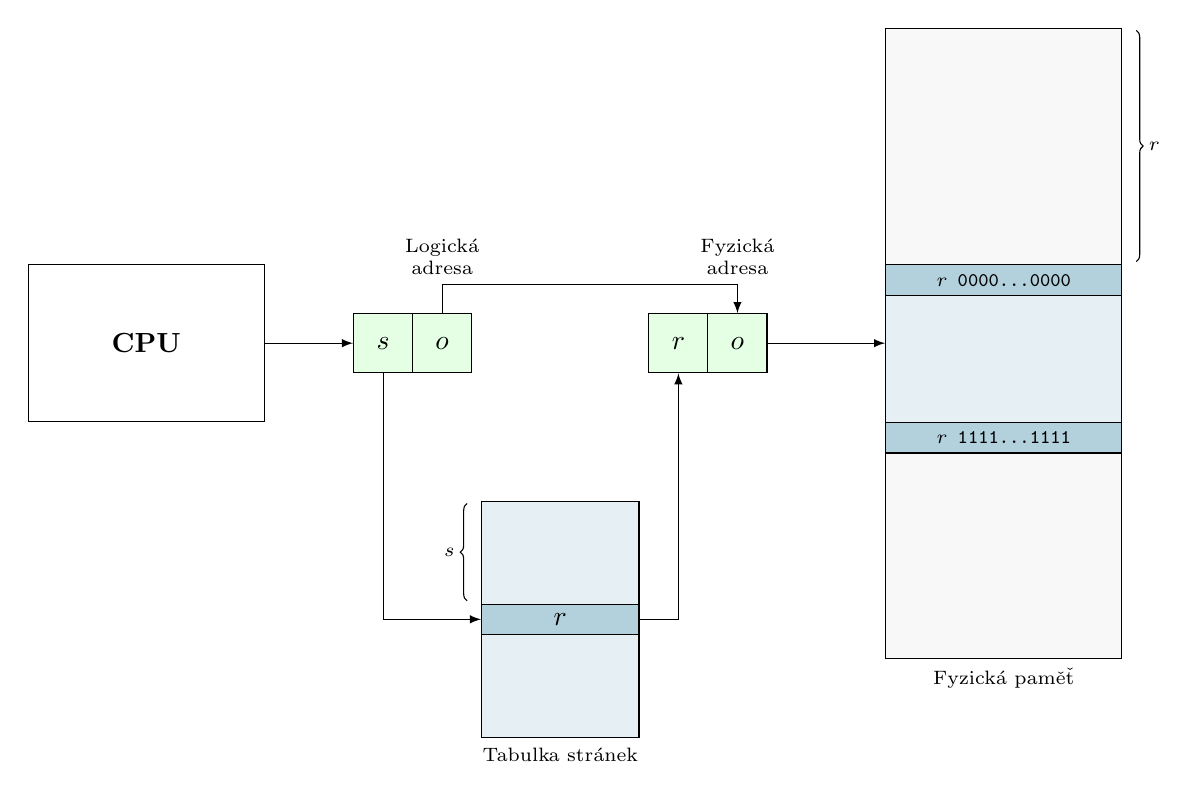
\begin{tikzpicture} [
        %font=\small,
        cpu/.style={draw, minimum width=3cm, minimum height=2cm, align=center, font=\bfseries},
        reg/.style={draw, minimum width=2.75cm, minimum height=1.75cm, align=center},
        mem/.style={draw, minimum width=3cm, minimum height=8cm, fill=themeGrey!5},
        mem check/.style={draw, diamond, align=center, font=\scriptsize},
        mem block/.style={draw, anchor=north, minimum width=3cm, minimum height=3cm, fill=themeBlue!10},
        sum address/.style={draw, circle, align=center, font=\scriptsize, scale=2},
        limit error/.style={below, minimum width=2cm, align=center, font=\scriptsize},
        label address/.style={midway, above, align=center, font=\scriptsize},
        label LAP/.style={right, font=\scriptsize, text=themeBlue},
        label mem/.style={above, font=\bfseries},
        % New styles:
        label page table/.style={below, font=\scriptsize, minimum width=1cm},
        addr block/.style={draw, minimum size=.75cm, fill=green!10},
        page table/.style={draw, fill=themeBlue!10, minimum width=2cm, minimum height=3cm},
        page table frame/.style={draw, fill=themeBlue!30,minimum width=2cm},
        mem frame/.style={draw, fill=themeBlue!30,minimum width=3cm, font=\ttfamily\scriptsize},
        brace mirror/.style={decoration={brace,mirror,raise=5pt}, decorate},
        brace/.style={decoration={brace,raise=5pt}, decorate},
        label left/.style={font=\scriptsize, align=right, left=6pt},
        label right/.style={font=\scriptsize, align=left, right=6pt},
    ]

    \path node[cpu] (cpu) {$ \text{\lCPU} $};

    \path (cpu.east) ++(right:1.5cm) node[addr block] (p) {$ s $};
    \path (p.east) node[addr block, anchor=west, xshift=-\pgflinewidth] (o) {$ o $};
    
    \path (o) ++ (right:3cm) node[addr block] (f) {$ r $};
    \path (f.east) node[addr block, anchor=west, xshift=-\pgflinewidth] (o2) {$ o $};
    
    \path (o2.east) ++(right:3cm) node[mem] (mem) {};
    \draw (mem.south) node[label page table] {\PhysicalMemory};

    \draw[-latex] (o) -- ++(up:.75cm) node[above, align=center, text width=1cm, font=\scriptsize] {\lAddressLogical} to ($ (o2.north|-\tikztostart) $) node[above, align=center, text width=1cm, font=\scriptsize] {\lAddressPhysical}  -- (o2.north);
    \draw[-latex] (cpu.east) -- (p);
    
    \draw ($ (p.west)!.5!(o2.east) $) ++ (down:2cm) node[page table, anchor=north] (page table) {};
    \draw (page table.south) node[label page table] {\lPageTable};
    
   \draw ($ (page table.north)!.5!(page table.south) $) node [page table frame] (page table frame) {$ r $};
   \draw[-latex] (page table frame.east) -| (f);
   \draw[-latex] (p.south) |- (page table frame.west) ;
   \draw[-latex] (o2.east) -- (mem.west) ;
   
   \draw ($ (mem.north)!.4!(mem.south) $) node[mem frame] (frame 0) { $r$ 0000…0000 };
   \draw ($ (mem.north)!.65!(mem.south) $) node[mem frame] (frame 1) { $r$ 1111…1111 };
   
   \fill[themeBlue!10] ($(frame 0.south west) + (\pgflinewidth, 0) $) -- ($(frame 0.south east) - (\pgflinewidth, 0) $) -- ($(frame 1.north east) - (\pgflinewidth, 0) $) -- ($(frame 1.north west) + (\pgflinewidth, 0) $) -- cycle;
   
   \draw[brace mirror]  ($ (page table.north west) - (0, 1pt) $) --  node[label left] {$ s $} ($ (page table frame.north west) + (0, 1pt) $);
   \draw[brace]  ($ (mem.north east) - (0, 1pt) $) --  node[label right] {$ r $} ($ (frame 0.north east) + (0, 1pt) $);

  
    \end{tikzpicture}
\end{document}
